\section{Study 1: User Behavior on an Imaginary TypeBoard}

In this study, we collected data from participants' typing actions on a pressure-sensitive touchpad. The motivation was to investigate users' typing behavior on an imaginary touchscreen keyboard that prevents unintentional touch, based on which we could design the algorithm of unintentional touch prevention. Because (incorrect) feedback would affect users' behaviors, participants typed on a touchpad without any feedback in this study. Participants could not enter words by typing on the touchpad. Instead, they imagined that the desired words are inputted. Besides, participants needed to adapt their behaviors according to the imagination that the keyboard can prevent unintentional touch.

%本实验的目标是研究用户在想象中防误触键盘上的打字行为,从而指导触屏键盘防误触算法的设计。由于(不正确的)反馈可能会影响用户的输入行为,在本实验中,用户在无反馈的键盘上打字,用户不能真的键入字母,而是想象可以键入字母。另外,用户需要假想键盘可以防止误触,调整自己的打字行为。

\subsection{Participants}

We recruited 16 participants from the campus (aged from 19 to 26, M = 22.13, SD = 2.13, eight females). All the participants were right-handed and native Chinese speakers. They have used software keyboards on smartphones for not less than two years (M=7.50, SD = 2.25). All the participants were familiar with physical keyboards. Eight participants have ever used software keyboards on tablets.

\subsection{Design and Procedure}

Figure xx illustrates the experimental setting. There was a Sensel Morph \cite{Website-Morph} pressure-sensitive touchpad on the desk. We placed a Windows Surface tablet computer on the touchpad, covering half of the touchpad. We drew a QWERTY layout on the touchpad using highlighter pens. The devices were a substitute for the pressure-sensitive touchscreen, which is not available in markets yet. Participants filled in a Microsoft Word document to complete the experimental tasks. They touched on the tablet to select table cell and typed on the touchpad to pretend to enter words. The system recorded every touch and the screencast during the experiment.

【图:实验一的实验设置,包含子图:平板电脑+压力触控板=压敏平板电脑】

%图xx展示了实验的设置,桌子上放着一块morph-sensel压力触摸板,在板子的上半部分叠放了一个windows surface,我们用这个组合来模拟未来可以支持压力输入的平板电脑。用户可以根据自己的需求调整椅子的高度、压力触摸板和显示器的位置。压力触摸板上用荧光笔画上了26键Qwerty键盘布局,用于提示用户每个按键的位置。用户在这个系统中通过填写word文档的方式来完成文本输入任务,系统会记录用户每次触摸的信息,以及给实验过程录屏。

The experiment included four sessions of text input tasks: (1) filling in personal information, (2) short questions, (3) open-book examination, and (4) picture writing. The tasks were in Chinese. We counterbalanced the order of tasks using a balanced latin square. We did not include transcription as a task as many other text entry studies do \cite{2003-Metrics, 2003-Phrase, 2017-Word}, because our pilot study showed that participants seldom rested their fingers on the touchpad in a transcription task, resulting in low efficiency of obtaining unintentional touches. The detail of tasks is as follows:

%实验分为四个session,分别对应四个不同的文本输入任务:填写个人信息、描述个人爱好、模拟开卷考试和看图写话。我们通过拉丁方来平衡每个用户做这四个任务的顺序。我们不像大多数文本输入相关工作一样[xx,xx,xx],将誊写作为文本输入任务,因为我们通过预实验发现,用户在誊写任务中很少将手指放在键盘上,误触的采集效率不高。图xx展示了每个任务的例子,每个任务的具体描述如下。

\begin{enumerate}
	\item{\textbf{Filling in personal information:} There was a table of ten blanks about personal information, such as name and gender. Figure \ref{fig:study1_task}(a) shows the examples in Chinese and the corresponding translation. This assignment represented those tasks that require frequent switching between text input and cursor control. To protect privacy, participants felt free to fill in fake information. However, participants should remember what they intended to enter, which is crucial for the subsequent process of labeling data.}
	\item{\textbf{Short questions:} There was a table of ten short questions, such as "the favorite color" and "the best friend". Participants were allowed to fill in a fake answer.}
	\item{\textbf{Open-book examination:} The exam consisted of five hard questions, such as "what is the 50th element on the periodic table?". Participants could hardly know the answers, so they needed to search the Internet. This assignment represented the common task of browsing websites. Because the participants could not input words in the search engine, they said as they wrote, so the experimenter could replace them to enter the words.}
	\item{\textbf{Picture writing:} As figure \ref{fig:study1_task}(b) shows, participants described the picture in five sentences. This assignment represented the tasks of writing articles. Participants said as they wrote, so the experimenter could replace them to enter the words.}
\end{enumerate}

\begin{figure}[!tbh]
	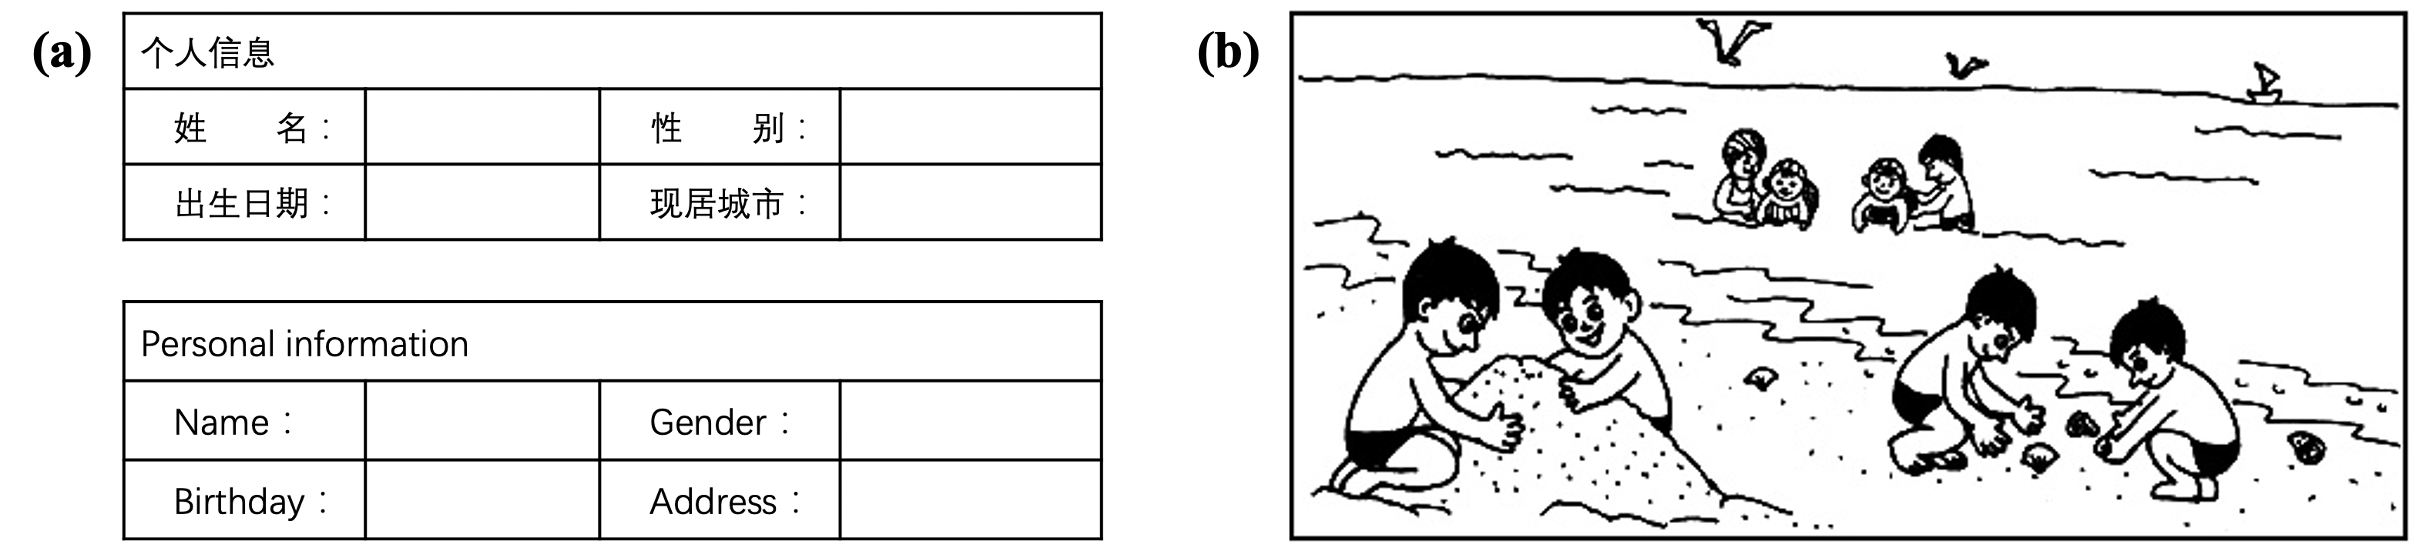
\includegraphics[width=0.9\linewidth]{figures/study1_task.png}
	\centering
	\caption{The illustration of experimental tasks. The left side shows the examples of task one (filling in personal information) in both Chinese and translation. The right side is the figure we used in task four (picture writing).}
	\label{fig:study1_task}
\end{figure}

%\begin{enumerate}
	%\item{\textbf{填写个人信息任务:}word文档中有一个表格,其中包含用户姓名、性别、专业等问题。用户操作触摸板(想象中的TypeBoard键盘)和平板电脑上的直接触摸填写表格。为了保护用户的隐私,用户可以填写错误的信息,前提是他能记住他填写的内容,以便标注时作为参考。用户需要点击平板电脑来切换表格中的焦点,然后再触摸板上敲击“输入”,想象所需字母被填写在了word文档中。该任务模拟了真实场景中,需要频繁切换键鼠操作的输入类型。}
	%\item{\textbf{描述个人爱好任务:}word文档中有一个问卷,其中包含“最喜欢的城市”、“最喜爱的食物”等个人喜好相关的问题。和任务一相同,用户通过键鼠配合操作完成问卷的填写。该任务模拟了真实场景中简单的问卷填写任务[xx]。}
	%\item{\textbf{模拟开卷考试任务:}word文档中包含若干有一定难度的知识性问题,如“比利时的首都在哪里”、“元素周期表中第50号元素时?”。在此任务中,用户很可能不知道问题的正确答案,此时她需要通过搜索引擎来得到答案。用户在使用搜索引擎时存在一个问题是,她输入的文字并不能真的上屏,此时我们要求用户边输入边把搜索的关键词说出来,实验者帮忙使用键盘完成搜索。both搜索的过程和填写试卷的过程是本实验采集的数据。该任务模拟了真实场景中常见的搜索引擎任务。}
	%\item{\textbf{看图写话任务:}word文档中包含了一张简笔画(如图xx的xx所示),用户需要根据这幅图写一个五句话的小作文。在此任务中,我们同样要求用户边说边写,实验者在一旁进行速记,这是为了在标注中给用户提高上下文。该任务模拟了真实场景中的办公场景[xx],这一类任务有着xx的特点。}
	%\item{\textbf{誊写任务:}word文档中包含了一句话,用户需要尽可能快地将这句话誊写五次。每个用户所誊写的句子都是不同的,都是从phrase-set[xx]中随机抽取。誊写任务是文本输入工作中最常见的评测任务,适用于评测输入法的输入效率上限。}
%\end{enumerate}

Before the experiment, the participant had five minutes to get familiar with the experimental requirement. In the warm-up phase, participants typed on the touchpad freely. We reminded the participants of two points. First, the keyboard did not provide any feedback. Participants could not enter words but imagined to enter words. As the Chinese text entry method involved word selection, participants assumed that the desired word is always the first in the candidate list. Second, users needed to imagine that the keyboard prevents unintentional touches and adjust their behavior according to this assumption. For example, they could rest their fingers on the keyboard while thinking.
%This is not mandatory. Participants could make choices as they wished.

%在实验开始前,用户有5分钟的时间自由地在本系统中熟悉实验的任务和要求,在热身的过程中,实验者让用户注意两点:第一,本实验的键盘不会提供任何反馈,用户不能键入字母,而是想象自己键入了字母。由于用户的母语是中文,在输入的过程中会涉及到选词,用户只需想象想要的单词总是在输入法候选词的第一位。第二,用户需要想象该键盘可以完美地防误触,并根据这一条件调整自己的输入行为,比如,在思考问题的时候可以将手指休息在键盘上。这种行为调整不是强制性的,用户可以根据自己的实际情况作出选择。

After each session, the participant labeled the data through an interactive program, which showed the touchpad capacitive images and the tablet screencast at the same time. As figure xx shows, there were red points on capacitive images that showed the touchpoints. Participants labeled the intended touches as green points. Participants were able to judge most touches because they could get context from the screencast. If participants were not sure, they labeled the touchpoints as blue points to remove the data. On average, participants spent five minutes finishing the text input tasks and spent 45 minutes labeling the data. Participants rested for five minutes between two sessions to avoid fatigue. The study lasted for 70 minutes.

【图:标注程序】

%在每个session结束后,用户需要通过一个交互式程序来标注刚刚所进行session的报点数据,该程序同时展示了实验过程中的录屏视频和压力板图像,用户需要结合录屏提供的上下文信息,标注压力板图像中的报点。如图xx所示,我们在平板电脑上外接了鼠标来提高用户的标注效率。压力图像中所包含的报点初始默认值为负例(误触),用红色点表示。用户若认为一个报点是正例(打字事件),则需要用鼠标左键将该点标为绿色;用户可以通过鼠标右键将报点重新标为红色;用户若不清楚该报点是正例还是负例,则需要用鼠标中键将该点标为蓝色,表示剔除出数据集。本实验的输入任务部分,四个session加起来大约需要15分钟,标注过程大约45分钟,每两个session之间休息5分钟时间来避免疲劳,实验总时长为80分钟。

\subsection{Apparatus}

As figure xx shows, we placed a Windows Surface tablet computer and a Sensel Morph pressure-sensitive touchpad \cite{Website-Morph} together as a substitute for the pressure-sensitive touchscreen. The Sensel Morph senses the position and the pressure level of touches. The Sensel Morph contains 185 x 105 sensor elements ("sensels") at a 1.25mm pitch. Each contact can sense approximately 30000 levels, ranging from 5g to 5kg. The maximal frequency of the Sensel Morph was 125Hz (8ms latency). We slowed the frequency down to 50Hz to fetch stable data. The Sensel Morph provides capacitive images and touchpoint information, including position, timestamp, touch area, pressure level, and shape. The device is so sensitive that almost every touch is recognized. Thus, in this paper, we identified unintentional touches among reported touchpoints while ignoring the Sensel Morph's missing touches.

%由于目前在商业上还没有具备压力感知能力的平板电脑(或是压力信息不灵敏[xx]),我们拼接了Morph Sensel压敏触摸板和Windows Surface平板电脑来模拟未来可能普及的压敏平板电脑(如图xx所示)。Morph Sensel是一个支持多点触摸的压敏触控板,可以感知触摸的位置和力度,185 x 105 sensor elements ("sensels") at a 1.25mm pitch,5g - 5kg sensing range per touch,Each contact can sense approximately 30,000 levels。Extremely Fast:High Speed Mode: 500 Hz (2 ms latency). morph sensel触摸板在提供电容屏图像的同时,还会提供报点信息,报点十分敏感,几乎所有的contact都会视为一次报点,因此在这份工作中,我们仅分析sensel的报点中哪些是误触,而不考虑morph sensel本身漏报的情况。

The size of the sensing area on the Sensel Morph was 240 mm x 138 mm. We used highlighter pens to draw a Qwerty layout on the touchpad, as figure xx shows. The Sensel Morph width (240mm) was shorter than the keyboard on a 15 inches MacBook (270mm). We removed some keys that are less frequently used, such as square brackets and the semicolon, so that the Qwerty layout could be placed in the Sensel Morph, while each key's size remained the same as Macbook. Because the Qwerty layout is changeable in the software keyboard, we did not leverage the layout as prior knowledge to recognize unintentional touch. The tablet computer was Windows Surface Pro6, with i7 Intel Core Processor. The program ran on the tablet at 50 FPS.

%传感区域的大小是240mm*138mm,我们在传感区域中央用记号笔画上了Qwerty布局,用来提示用户每个按键所在的位置。Morph Sensel的传感区域比15寸MacBook上的键盘(xx-mm*xx-mm)小一些,为了能在触摸板上画上Qwerty布局,而不对用户的打字行为造成太大的影响,如图xx所示,我们维持了MacBook键盘上每个按键的大小,并去除了本次实验中不会用到的符号键(如中括号和分号)。由于软键盘的布局可以多种多样,而我们希望做一个应用范围更广的防误触算法,因此我们不会将键盘布局作为先验知识应用在防误触算法当中。

\subsection{Result}

The dataset contains 12659 touches, excluding the ambiguous touches (0.18\%) in the labeling process. 67.5\% of the data were positive samples (intentional touches), while 32.5\% were negative samples (unintentional touches). Based on the data, we developed the TypeBoard in three steps, each contributing to solving one of the critical problems as follows:

\begin{enumerate}
	\item{\textbf{Model V1):} \emph{data processing.} There were some mislabeled data points because some participants misunderstood the concept of unintentional touches. We developed a naive Support Vector Machine (SVM) model to identify unintentional touch. If there was a vast difference between the predicting results and the labels, we asked the participants to relabel the suspicious data points through e-mails.}
	\item{\textbf{Model V2):} \emph{filtering multiple fingers resting.} Observation suggested that multiple fingers resting was the most frequent (> xx\%) unintentional touch, where users rested more than two fingers on the screen. We added targeted criteria into the SVM model to filter out multiple fingers resting.}
	\item{\textbf{Model V3):} \emph{understanding the user behavior.} We analyzed the fail cases of Model \textbf{V2} to understand those user behaviors that challenged the algorithm, based on which we further improved the SVM model.}
\end{enumerate}

\begin{table}[!tbh]
	\caption{The features we fed into the SVM model and the accuracy among model versions. For the features except "the relationship to recent/nearby touches", we extracted the temporal features over frames, including maximum, minimum, mean, skewness, and kurtosis.}
	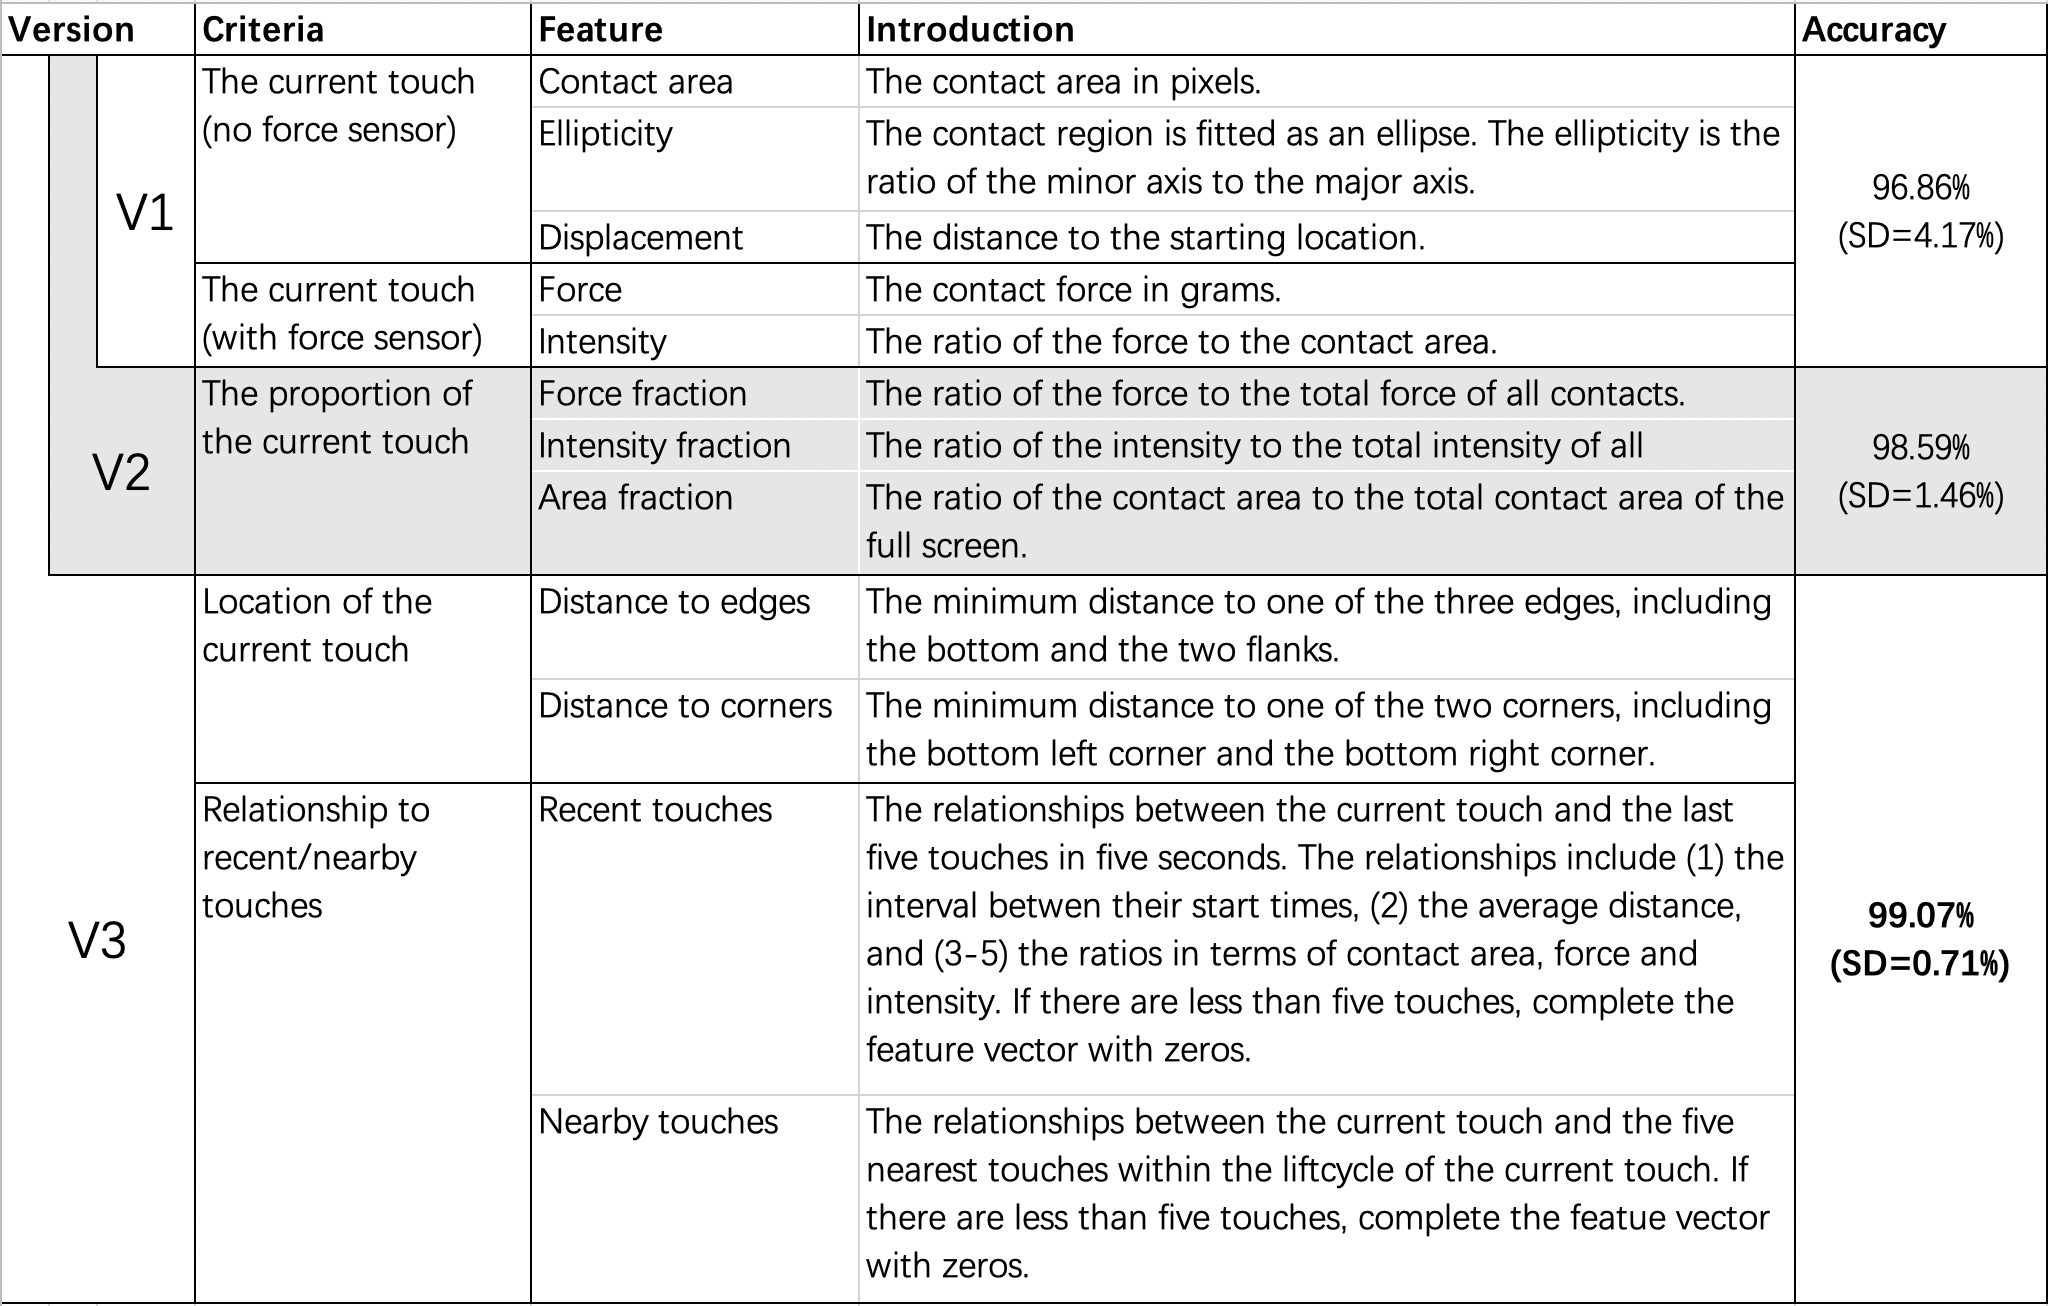
\includegraphics[width=1.0\linewidth]{figures/features.png}
	\centering
	\label{tab:study_features}
\end{table}

Table xx shows the feature vector we used to train the SVM model in each step and the recognition results. In the remainder of this subsection, we introduced the unintentional touch identification model in detail.

%Because some participants misunderstood the concept of unintentional touches when labeling, there were some mislabeled data points. We trained a simple machine learning model (version 1) to process the data. If there were too many differences between the labels and the predicting results, we asked the participants to relabel the suspicious data points.

\subsubsection{Model  V1: naive model for data processing}

In the first step, we trained a naive SVM model to identify unintentional touch using straightforward features. We sampled the first five frames (100 ms) of each touch. If the touch duration is shorter than five frames, we sampled the whole touch. As table xx (\textbf{V1}) shows, we extracted features from the samples as follows: for the contact area, ellipticity, displacement, force, and intensity over frames, we calculated the temporal features, including maximum, minimum, mean, skewness, and kurtosis. Then, we concatenated these values to obtain a feature of 25 dimensions and trained an SVM binary classifier, namely Model \textbf{V1}. We balanced positive and negative samples in weight.

%如表格xx所示,我们首先开发了一个简单、直观的机器学习方法(version-1)。我们采样每个报点后前5帧(100ms)的数据作为样本,如果一次点击事件的持续时间不足五帧,则将整个点击事件作为样本。然后,我们通过以下方法来提取样本的特征:对于报点面积、椭圆度、位移、压力和压强这五个数值,分别计算它们在五帧中的时序特征(最大值、最小值、平均值、偏度和峰度),排列成一个25维的特征向量,最后使用SVM二分类器进行分类,训练时平衡了正负样本的权重,也对每一维特征分别先进行归一化。

We used the model to simulate the dataset. We found that some participants misunderstood the concept of unintentional touches, for example, regarding incorrect character inputs as unintentional touches. We asked the participants to relabel the suspicious data points through e-mail. After the label correction, we had xx data points, including xx.x\% positive samples and xx.x\% negative samples. Leave one out cross-validation shows that the accuracy of Model \textbf{V1} was 96.86\% (SD=4.17\%). 

%For comparison, if we did not have the force signal (i.e., the regular touchscreen devices), the accuracy would reduce to 92.30\% (SD=4.88\%). The result shows that the force signal is important for unintentional touch rejection (F,p).

%我们用这个简单的机器学习方法来预测实验一中采集的数据。我们发现,有的用户在标注的时候对误触的理解出现了偏差,例如将打错字母标注成无意触摸,对于这种实验者认为有可疑的数据点,我们都通过邮件的方式请当事人用户重新标注。在所有数据都被检查无误之后,我们共有xx个数据点,其中正例占xx.x\%,负例占xx.x\%。至此,我们认为数据集的标注准确无误。

%留一法显示版本1的模型对误触的识别准确率达到96.86\%,作为对比,如果我们不利用压力信息(版本0),准确率仅为92.30\%。这一结果说明,压力信号在tablet键盘防误触方面起了非常重要的作用(F,p)。

\subsubsection{Model V2: filtering multiple fingers resting}

Observation showed that most unintentional touches (xx.x\%) were caused by multiple fingers resting, where users rested no less than three fingers on the screen simultaneously. The resting fingers contact the screen one after another. After the first touch, the following touches come within 100 ms in most instances. In xx.x\% cases, the second finger touches within 100 ms, while in xx.x\% cases, the third finger also touches within 100 ms. Because our model has a latency of 100 ms, the model has a big chance to realize that multiple fingers are resting. Thus, we could design targeted features to filter out the unintentional touches caused by multiple fingers resting.
We added a series of features in Model \textbf{V2} to deal with this problem. The criterion was the proportion of the touch's pressure, intensity, and contact area among all touches. Table xx (\textbf{V2}) shows the details. Leave one out cross-validation shows that Model \textbf{V2} increased the recognition accuracy to 98.59\%.

%在一次手指误触的生命周期中,若屏幕上屏幕上出现过三个或者以上的手指误触,则我们认为该误触是多指休息行为造成的。在一次多指休息行为中,不同的手指不可能恰巧同时触碰到屏幕,这些手指是依次接触到屏幕的。我们的识别算法有100毫秒的识别延迟,幸运的是,在这100ms的时间内,在xx.x\%的情况下第二根手指参与其阿红,在xx.x\%的情况下有三根或以上的手指参与其中。也就是说,在我们需要作出判断的时候(接触后100毫秒),系统有机会认识到这是一次多指休息行为了,我们可以设计专门的特征来排除。

% 观察发现,多指同时休息是最常见的误触行为,占所有无意报点总数的x0\%以上。为了解决这个瓶颈问题,我们在模型中新增了一系列表达“本次点击在所有点击中所在的比重”的特征(table xx - V2),这些特征包含本次点击的接触面积、压力和压强占全屏总接触面积、总压力和总压强的比例。对于这三个数值,同样需要计算时域信息,即五帧中的最大值、最小值、平均值、偏度和峰度,共新增15维特征。重新训练得到新的模型(版本2),留一法显示准确率上升至98.59\%。

\subsubsection{Model V3: understanding the user behavior to  improve the model}

We analyzed the fail cases of Model \textbf{V2} to understand those user behaviors that challenged the model. The error rate of Model \textbf{V2} was 1.41\%, including xx.x\% false positives and xx.x\% false negatives. The false positives referred to the misrecognized unintentional touches, while the false negatives were the missing intentional touches. As table xx shows, we classified the fail cases into 16 categories. We counted each kind of fail case, discussed the reasons, and gave possible solutions. For the fail cases with a white background in the table, humans (the researchers) could judge their intentions without extracting contextual information from the experiment screencast. That is, the machine should have correctly predicted if it is as smart as a human. For these cases, we proposed features to improve the model. Here are some examples.

%为了进一步提高模型的预测准确率,我们分析了V2版本模型的错例,并推测这些错例是由怎样用户行为导致的。如表格xx所示,有xx.x\%的错例(白色背景部分)是人类(实验者)能够人工分析出正确结果的,我们可以为这些错例设计针对性的特征,从而提高模型的预测准确率。这些错例中比较典型的例子有:

\begin{enumerate}
	\item{\textbf{EG1):} \emph{Hypothenar eminence.} As figure \ref{fig:fail_case_examples}(a) shows, the hypothenar eminence refers to a group of muscles of the palm that control the motion of the little finger, while the thenar eminence is the group of muscles on the palm at the base of the thumb. Both the two eminences may contact the touchscreen when a user is typing. In particular, the touches caused by the hypothenar eminence are usually heavy and intensive, which is easy to confuse with intentional touches. Fortunately, these touches are in the bottom left and the bottom right corners. Thus, the distance to the closest corner could be a powerful feature to reject these unintentional touches.}
	\item{\textbf{EG2):} \emph{Continuous touches.} When a user continuously typed on the same key (e.g., the delete key), the following touches were lighter than the first touch (F,p). Among the continuous touches, the average pressure of the first touch was xx.x g, while the average pressure of the following touches was xx.x g. Because the following touches are light, they are likely to be recognized as unintentional touches. Information of recent touches help to correct this fail case.}
	\item{\textbf{EG3):} \emph{One-hand typing.} As figure \ref{fig:fail_case_examples}(b) shows, sometimes the participant typed with one hand while resting the other hand on the touchscreen. In this situation, the Model \textbf{V2} mistakenly believed that all the touches were unintentional touches caused by the multiple fingers resting behavior. We added information of nearby touches to correct this fail case because the typing finger is usually far away from the resting fingers.}
\end{enumerate}

\begin{figure}[!tbh]
	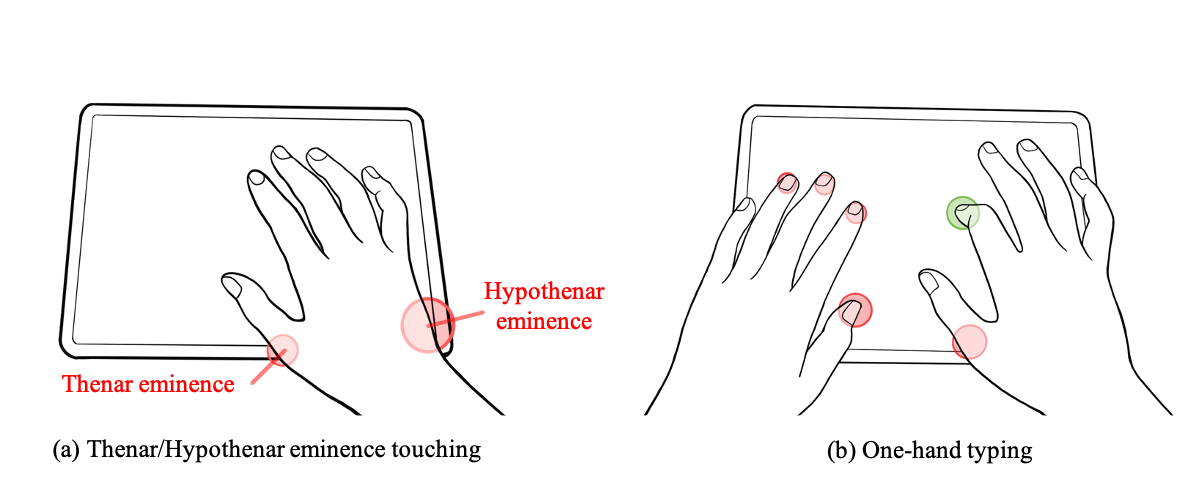
\includegraphics[width=1.0\linewidth]{figures/fail_case_examples.png}
	\centering
	\caption{The examples of fail cases. The fail cases reveal those user behaviors that challenged the algorithm.}
	\label{fig:fail_case_examples}
\end{figure}

% Table generated by Excel2LaTeX from sheet '写在论文中的中等粒度分类'
\begin{table}[htbp]
  \centering
  \caption{The fail cases of Model \textbf{V2}. The "N" column refers to the counting of each case.}
    \begin{tabular}{|p{8.5em}|p{21em}|r|p{10.5em}|}
    \toprule
    \textbf{Cases} & \textbf{Introduction} & {\textbf{N}} & \textbf{Helpful features?} \\
    \midrule
    \rowcolor[rgb]{ 1,  .902,  .6} \multicolumn{4}{|l|}{\textbf{False Positives}} \\
    \midrule
    Hypothenar eminence (figure \ref{fig:fail_case_examples}a) & The hypothenar eminence usually contacts the screen while typing. & 23    & Touchpoint location, e.g., nearing the corners? \\
    \midrule
    Thenar eminence (figure \ref{fig:fail_case_examples}a) & The thenar eminence usually contacts the screen while typing. & 2     & Touchpoint location, e.g., nearing the bottom edge? \\
    \midrule
    Repeated reporting (spatial) & A touch is misrecognized as two touches when the contact area is large. & 12    & Info. of nearby touchpoints. \\
    \midrule
    Repeated reporing (temporal) & A touch is misrecognized as two touches if the touch is nearly released midway. & 3     & Info. of recent touchpoints. \\
    \midrule
    Edge touch & Users trigger unintentional edge touch when adjusting the placement of devices. & 7     & Touchpoint location, e.g., nearing the flanks? \\
    \midrule
    Two fingers resting & The user rests two fingers on the screen. & 3     & Info. of nearby touchpoints. \\
    \midrule
    Extra touchpoint (light) & When inputting, users trigger extra touchpoints, which are lighter than the recent intentional touches. & 9     & Is this touch lighter than the recent touches? \\
    \midrule
    Slide & A slide is less likely to be an intentional keystroke. & 7     & Touchpoint displacement. \\
    \midrule
    \rowcolor[rgb]{ .949,  .949,  .949} One finger resting & Users rest one finger on the touchsreen, which is indistinguishable from an intentional touch. & 9     & No solution. \\
    \midrule
    \rowcolor[rgb]{ .949,  .949,  .949} Extra touchpoint (heavy) & When inputting, users trigger extra touches heavily, which seems like an intentional touch. & 15    & No solution. \\
    \midrule
    \rowcolor[rgb]{ 1,  .902,  .6} \multicolumn{4}{|l|}{\textbf{False Negatives}} \\
    \midrule
    Continuous touches & When a user continuously type on the same key (e.g., the delete key), the following touches will be lighter. & 13    & Info. of recent touchpoints. \\
    \midrule
    Rollover-typing & The next key is pressed before the previous is released \cite{2018-Observations}. & 12    & info. of recent touchpoints. \\
    \midrule
    One-hand typing & The user types with one hand, while the other hand is resting on the screen. This case is similar to multiple fingers resting. & 6     & info. of nearby touchpoints. \\
    \midrule
    Palm touch & The use types a key when the palm is resting on the screen. If the palm touch is detected as multiple fingers, this case is similar to multiple fingers resting. & 5     & info. of nearby touchpoins, e.g., is this touch near other touches? \\
    \midrule
    \rowcolor[rgb]{ .949,  .949,  .949} Light touch & The very light but intended touch, which is indistinguishable from an unintentional touch. & 46    & No solution. \\
    \midrule
    \rowcolor[rgb]{ .949,  .949,  .949} Small contact area & The intended touch with a very small contact area. This seems like an unintentional touch. & 6     & No solution. \\
    \bottomrule
    \end{tabular}%
  \label{tab:fail_cases}%
\end{table}%

%(1)V2版模型有些时候会把小鱼际的误触判定为有意点击。我们发现,用户的小鱼际误触主要集中在触摸屏的左下角和右下角。因此,我们给模型添加上了一系列"Distance-to-corners"的特征,这样一来,模型将会降低在小鱼际处识别出有意点击的概率。
%(2)用户在连续点击同一个按键时(比较常见的是删除键),后续的点击可能会变得很轻,使得它的力度看上去更像是一个无意点击,V2版模型不能很好地处理这个问题。因此,我们给模型添加上了一系列"ralationship-to-recent-touches"的特征,这样一来,连续点击即使变得更轻,也能被正确地识别成有意点击。
%(3)有的用户可能会出现单手打字,另一只手指放在屏幕上休息的行为,这种情况下V2版模型可能认为所有手指都是在参与多指休息。因此,我们给模型添加上了一系列"ralationship-to-recent-touches"的特征,这样一来,如果本次点击距离同屏的其它点击距离较远,则可解释为one-hand-typing行为,从而被正确识别为有意点击。

However, for the fail cases with gray background in table \ref{tab:fail_cases}, humans (the researchers) could judge their intentions without watching the experiment screencast. We deemed that these fail cases are inevitable because the machine can not know what the user will enter in advance. Here are some examples. First, sometimes the participant rested one finger on the touchscreen heavily, indistinguishable from an intentional touch. Second, the participant performed a very light touch during entering a word, which is indistinguishable from an unintentional touch. Thus, the model's accuracy has a certain upper limit (roughly xx.x\% in this dataset), while our goal is to approach it.

%然而,有xx.x\%的数据(灰色背景部分),是人类也不能在不看上下文(实验录屏)的情况下分析出正确结果的,我们认为这部分的误触和漏报是不可避免的。这一类错例的典型例子有:(1)一只手指休息在键盘上,且力量很大,这种行为和用户打单词的第一个字母的行为非常相似(2)打字过程中出现一次很轻的有意点击,这种行为和打字过程中的误触非常类似。我们认为系统无法避免这种误触,也就是说,即使是人工判断每次点击是否有意,错误率也不低于xx.x\%(V2错误率 * V2错例中人类无法分辨的部分)。

According to the user behaviors summarized in table \ref{tab:fail_cases}, we added two criteria in the model training. The first one is the location of the touch, including the minimum distances to the edges and the corners. We did not leverage the prior knowledge of the keyboard layout because the software keyboard layout is changeable, while we wanted a universal model. The second criterion is the relationships between the current touch and the recent/nearby touches. The features in detail are in table xx (\textbf{V3}). The Model \textbf{V3} used all the features in table xx. We concentrated these features to form a vector of 100 dimensions and trained an SVM binary classifier. Leave one out cross-validation showed that the accuracy was 99.07\%. The error rate was 0.93\%, including xx.x\% false positives and xx.x\% false negatives. So far, we have obtained a model with high recognition accuracy. However, as we said in the introduction, the data collected in study one did not represent the user behavior on the software keyboard with unintentional touch prevention, so we named Model \textbf{V3} as semi-finished TypeBoard. In study two, we collected the user behavior on the semi-finished TypeBoard and then used the new data to improve the model.

% We used previous work as baseline \cite{2013-TapBoard}, where every touches that last for more than 450 ms or move father than 15 mm are identified as unintentional touches. We adjusted the thresholds to xx ms and xx mm so that the baseline performed the best on our dataset. Our result (99.07\%) surpassed the baseline (xx.xx\%). In real use, our system calls the classifier once a touch has lasted for five frames or is released in advanced. The system reports the touchpoint if the prediction result is positive. The delay of our method is 100 ms. For comparison, the baseline can only judge a touch when it is released.

%99.07\%的识别准确率远远超过了先前工作[xx]对打字过程中误触的识别准确率,在我们的数据集下,先前工作所使用的阈值方法(时间<xxms,位移<xx厘米)准确率仅为xx.x\%,即使重新调整阈值使其在我们的数据集下达到最优(时间<xxms,位移<xx厘米),准确率也仅为xx.x\%,因此我们的算法在准确率上成倍地提高了已有工作的水平。In real use, the system calls this classifier once a touch is released or has lasted for five frames, and reports the touchpoint if the prediction is positive. The delay is within 100ms. 延迟问题也是我们的算法对比于baseline的一大改进,相比之下,baseline只能在点击事件抬起时做出判断。

%针对表格xx中总结出来的用户行为,我们在模型中新增了两大类特征,分别是本次点击的坐标(V3)和本次点击与时空临近点击之间的关系(V4),最终,新模型的预测准确率达到了99.07\%,十分接近人类判断的准确率。至此,我们认为已经得到了实验一数据下的最佳结果。

%\begin{figure}[!tbh]
%	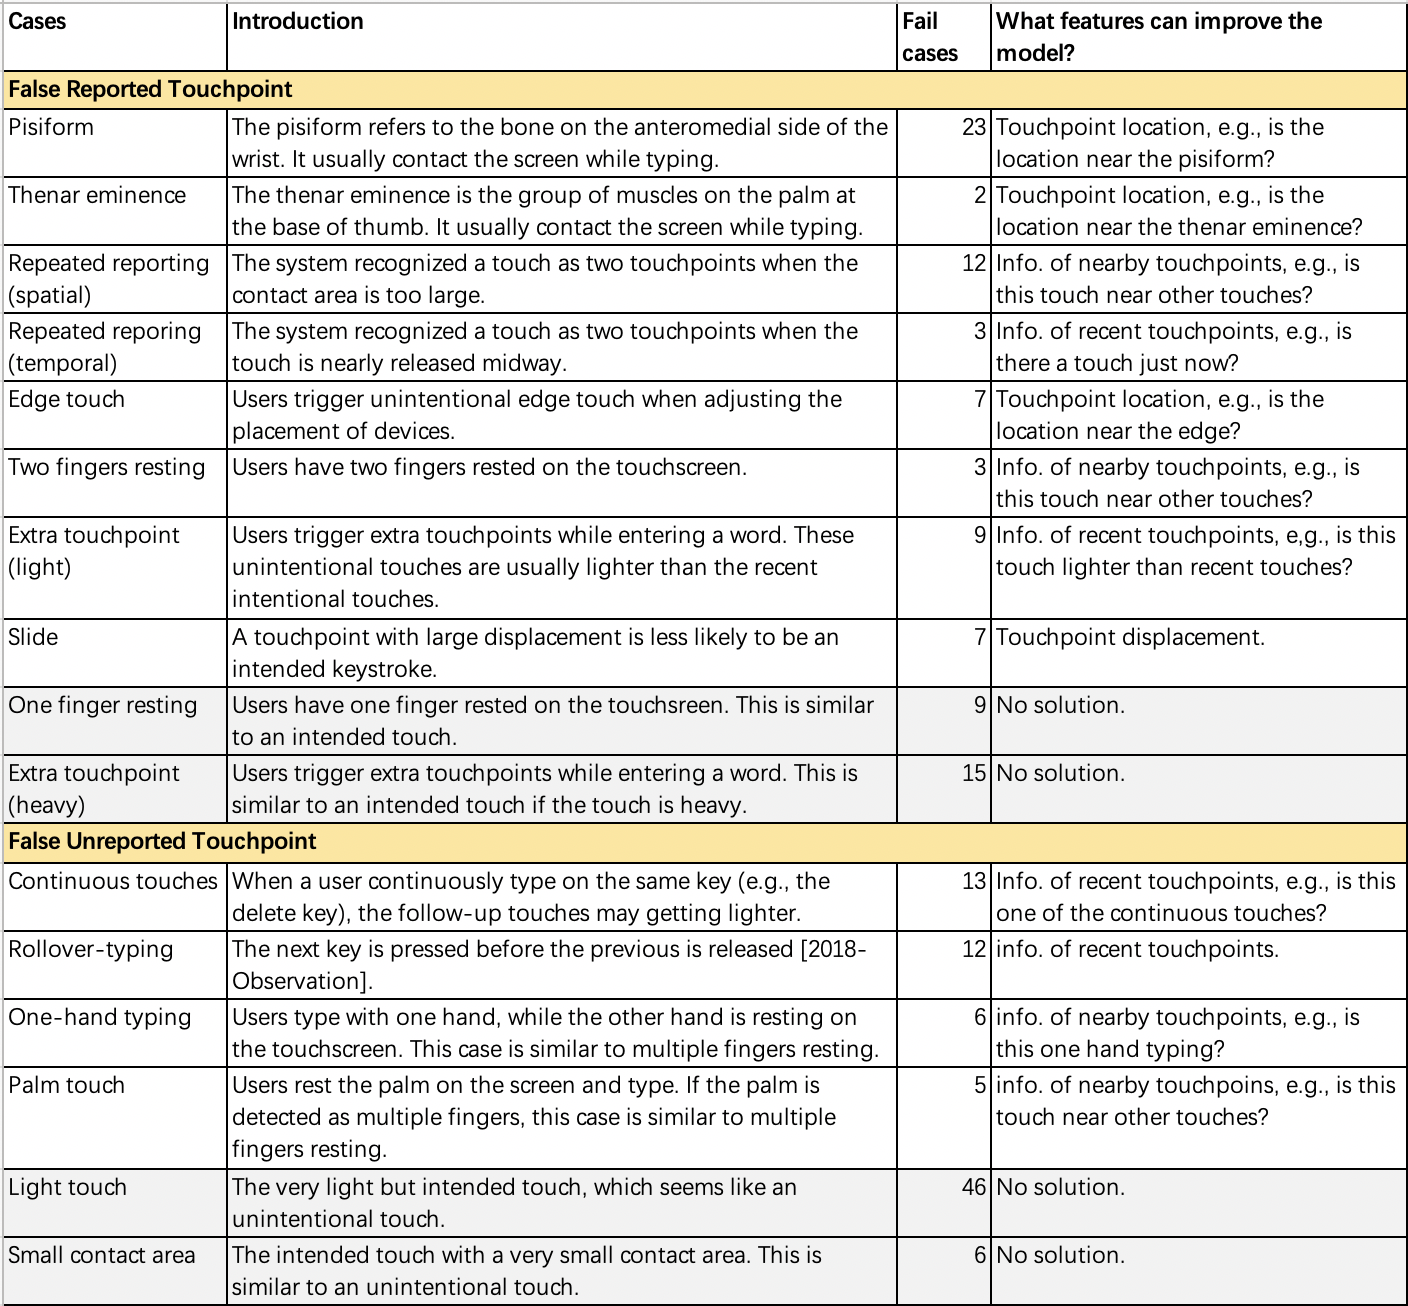
\includegraphics[width=1.0\linewidth]{figures/fail_cases.png}
%	\centering
%	\caption{The fail cases of Model \textbf{V2}. The "fail cases" column refers to the number of false positive/negative touches. }
%	\label{fig:fail_cases}
%\end{figure}

%We have three conclusions in this experiments. First, participants were willing to rest their fingers on the touchscreen that can reject unintentional touches in imaginary. Hereby, we proposed a hypothesis to be verified, where users are willing to rest their fingers on a real TypeBoard. Second, the force signal is important for rejecting unintentional touches in the text entry task. Third, most unintentional touches (>99\%) can be identified by spatial-temporal features of the signals on a force-sensitive touchsreen keyboard.

%在本实验中,我们能得到三个基本结论:(1)在想象中可以防误触的键盘上,用户十分乐意将手指休息在触屏上。由此我们提出一个假设:如果实际上存在一个能够极大概率拒绝误触,用户也会乐意将手指休息在触屏上。我们会在后续的实验中验证该假设。(2)压力信息对tablets打字防误触算法的提高是显著的。(3)大部分典型的误触行为都可以根据压力屏上触点的时空特性识别出来,准确率超过99\%。除了以上基本结论外,我们还讨论了下列问题:

%为什么选取报点后5帧的数据?首先做出判断的时间和准确率是tradeoff,延迟越大,机器学习的准确率就越高,但同时用户体验受到延迟的影响就越大。为了找到一个平衡点,我们分析了延迟为3帧~7帧的情况,结果如图xx所示,xxx。考虑到用户在点击时能感知到100ms的延迟[xx],我们选取了5帧(100ms)作为算法的判定时机。

%\subsubsection{What we found about user behavior?} Here are some conclusions. First, the unintentional touches mainly contains three categories, including multiple fingers resting (xx.x\%), palm touches (xx.x\%) and others (mostly mistaken touches during input, xx.x\%). Second, the text entry task has significant effect on the amount of unintentional touches (F, p). Bonferroni-corrected post-hoc tests showed significant differences between the following task pairs: xx-xx (p<), xx-xx (p<), and xx-xx (p<). Thus, we suggest that studies of unintentional touch should consider the variety of task. We will discuss the user behavior in details in the next study, because it is more meaningful to analyze the user behavior on a real TypeBoard.

%用户行为有什么规律?在这里,我们直接给出几个结论:(1)误触点主要由三部分构成,分别是多指休息(占xx.x\%),手掌误触(占xx.x\%)和输入间误触(xx.x\%),还有其它情况如用户主观打错没有纳入统计。(2)不同任务对用户无意点击数量有显著影响,其中有差异的任务对有xx,这说明,相关工作中讨论不分任务地讨论误触问题是存在问题的。我们不对以上规律作展开讨论,因为实验一采集的是用户在想象中的防误触键盘上的打字数据,该数据的代表性不强。在下一个实验当中,我们将会采集用户在model-version-4上的打字行为,迭代式地继续改进误触识别算法,并更加详细地探讨用户的行为。
